\documentclass[report]{article}
\usepackage{pagecolor,lipsum}
\usepackage{ragged2e}
\usepackage{graphicx}
\usepackage{subcaption}
\usepackage{enumitem}
\usepackage[none]{hyphenat}

\usepackage{tocloft}

\usepackage[norsk]{babel}
\usepackage[bottom=8em]{geometry}
\usepackage{amsmath}
\usepackage{graphicx}

\usepackage{ifluatex}
\ifluatex
%% Ved bruk av lualatex %%
\usepackage{fontspec}
\setmainfont{Linux Libertine O}
%%%%%%%%%%%%%%%%%%%%%%%%%%%
\else
%% Ved bruk av pdflatex %%
\usepackage[utf8]{inputenc}
\usepackage{libertine} % linux libertine font
%\usepackage[libertine]{newtxmath}
\usepackage[T1]{fontenc}
%%%%%%%%%%%%%%%%%%%%%%%%%%%
\fi

\usepackage{parskip}
\usepackage{xcolor}
\usepackage{lipsum}
\usepackage{calc}
\usepackage[labelfont=bf,textfont=normal,justification=justified,singlelinecheck=false,width=0.9\textwidth]{caption}

\usepackage{booktabs}
\usepackage{longtable}
\usepackage{rotating}
\usepackage{tabularx}

\usepackage{fancyhdr}


\definecolor{skde}{HTML}{0099e5}
\definecolor{skdelys}{HTML}{0099e5}
\definecolor{newcolor}{HTML}{333333}
\definecolor{number}{HTML}{D5D5D5}

%\definecolor{skde}{RGB}{0,79,158}
%\definecolor{skdelys}{RGB}{122,178,220}

\usepackage{sectsty}
\chapterfont{\color{skde}}  % sets colour of chapters
\sectionfont{\color{skde}}  % sets colour of sections
\subsectionfont{\color{skde}}  % sets colour of sections
\subsubsectionfont{\color{skde}}  % sets colour of sections

\usepackage[colorlinks, citecolor=number, linkcolor=number, urlcolor=number]{hyperref}


% Flere figurer per side etc
\renewcommand{\topfraction}{0.95}	% max fraction of floats at top
\renewcommand{\bottomfraction}{0.95}	% max fraction of floats at bottom
\renewcommand{\textfraction}{0.05}	% allow minimal text w. figs
\renewcommand{\floatpagefraction}{.8} %only pages with more than 80% of floats, will become pure float-only pages. The default is 0.6



\title{JPE\_Twitter} % tittel
\newcommand{\subtitle}{Aplicación Splunk para Mineria de Twitter} % undertittel
%\newcommand{\sammendrag}{Sammendrag legges inn her. \lipsum*[2]} % sammendrag
\newcommand{\sammendrag}{\justify El presente documento fue pensado, diseñado y redactado \'unica y exclusivamente para la comprensi\'on general del aplicativo JPE\_Twitter, por lo tanto, no puede ser editado y distribuido sin la previa autorizaci\'on escrita de su autor.}
\newcommand{\notatnummer}{Mayo de 2019} % dato for rapport (erstatter notatnummer)

\author{%
    Juan Alejandro P\'erez Chand\'ia \\
    Ingeniero Inform\'atico\\
    jalejandro.ingeniero@gmail.com
}

\newcommand{\hoydestrek}{125pt} % kommer an på antall forfattere

\definecolor{text}{HTML}{D5D5D5}
\definecolor{background}{HTML}{222222}

\usepackage{caption}
\usepackage[font={color=text,bf},figurename=Fig.]{caption}

	
\usepackage{geometry}
\geometry{top=2cm, bottom=2cm}
\usepackage{amsmath}
\usepackage{tikz}
\usepackage{epigraph}

\renewcommand\epigraphflush{flushright}
\renewcommand\epigraphsize{\normalsize}
\setlength\epigraphwidth{0.7\textwidth}

%\DeclareFixedFont{\titlefont}{T1}{ppl}{b}{it}{0.5in}
\DeclareFixedFont{\titlefont}{T1}{ppl}{}{}{0.5in}
\DeclareFixedFont{\subtitlefont}{T1}{ppl}{}{}{0.2in}

\makeatletter                       
\def\printauthor{%                  
    {\large \@author}}
\let\printtitle\@title
\makeatother


\newcommand\titlepagedecoration{%
\begin{tikzpicture}[overlay]%[remember picture,overlay,shorten >= -10pt]
%\draw[opacity=0.05,white, fill=skde] (-15,20) circle (125pt);
%\draw[opacity=0.15,white, fill=skde] (2,20) circle (4cm);
%\draw[opacity=0.1,white, fill=skdelys] (2,8) circle (4cm);
%\draw[opacity=0.1,white, fill=skdelys] (-10,8) circle (4cm);
%\draw[opacity=0.1,white, fill=skdelys] (2,-4) circle (4cm);
%\draw[opacity=0.05,white, fill=skde] (-15,20) circle (125pt);
\draw[opacity=0.15,white, fill=newcolor] (2,20) circle (4cm);
\draw[opacity=0.1,white, fill=newcolor] (2,8) circle (4cm);
\draw[opacity=0.1,white, fill=newcolor] (-10,8) circle (4cm);
\draw[opacity=0.1,white, fill=newcolor] (2,-4) circle (4cm);
\end{tikzpicture}%
}



\pagestyle{fancy}
 
\fancyfoot{}
\renewcommand{\footrulewidth}{0pt}
\renewcommand{\headrulewidth}{0pt}
% \fancyfoot[RO,LE]{\centering \color{text}\thepage}
\fancyfoot[R]{\centering \color{text}\thepage}
\fancyhead{}
\fancyhead[L]{}
\fancyhead[C]{}

\date{\today}




% 			S T A R T   D O C U M E N T
\begin{document}
\renewcommand*\contentsname{\color{skde}Contenido}
\pagecolor{background}
\color{text}
\sloppy 

\begin{titlepage}

%\newgeometry{bottom=2cm}%, top=2cm}

\vspace*{1cm}

\noindent
{\textcolor{skde}{\titlefont \printtitle{}}}\par
%\textcolor{skde!70}{\rule{\widthof{\printtitle{}}}{10pt}}

\vspace*{0.5cm}
{\subtitlefont \subtitle}

\vspace*{1cm}
\epigraph{\sammendrag}{\notatnummer}
\null\vfill
\vspace*{1cm}
\noindent
\hfill
\begin{minipage}{0.39\linewidth}
    \begin{flushright}
        \printauthor
    \end{flushright}
\end{minipage}
%
\begin{minipage}{0.02\linewidth}
\null
\end{minipage}
\begin{minipage}{0.02\linewidth}
    \rule{1pt}{\hoydestrek}
\end{minipage}
\titlepagedecoration


\hfill

\begin{minipage}{2in}

\includegraphics[width=0.8\textwidth]{img/jp_gris}
\end{minipage}
\hfill
\begin{minipage}{3in}
\begin{flushright}
\textcolor{skde}{
\href{http://www.jpengineer.cl}{\textcolor{skde}{JPEngineer \textcopyright}}
}
\end{flushright}
\end{minipage}

%\restoregeometry

\end{titlepage}
\addtocounter{page}{1}
% \begin{large}

\section{Introducci\'on}
JPE\_Twitter es una aplicaci\'on Splunk desarrollada en Python, cuya finalidad es la miner\'ia en Twitter e integraci\'on completa con la herramienta de an\'alisis de logs anteriormente mencionada. Con JPE\_Twitter podr\'as extraer de Twitter informaci\'on relevante basada en filtros de palabras, frases, oraciones, hashtag, etc. y obtener datos que indican lo que est\'a pasando en un negocio o servicio determinado en dicha red social, construyendo as\'i, una base de desarrollo para el an\'alisis de sentimiento en Twitter.
\newpage
\tableofcontents
\thispagestyle{empty}

\newpage
\section{Generalidades del Desarrollo}

El aplicativo esta desarrollado en python 2.7, con la finalidad de compartir la instalación base de python de la plataforma Splunk (6.x o superior) y cuenta con cinco m\'odulos esenciales:
\newline
\begin{itemize}
\item {\bf config :} El aplicativo cuenta con un archivo de configuraci\'on llamado \textit{twitter.conf}, donde el modulo config l\'ee y escribe los p\'arametros necesarios para la autentificaci\'on del listener con la API de Twitter, configuraci\'on base de logs, encriptaci\'on, entre otros.

\item {\bf security :} Para la seguridad de datos sencibles (Token autenticaci\'on), este m\'odulo cuenta con lo necesario para cifrar y descifrar en base a la clave que el usario determine en la configuraci\'on de los token en Splunk.

\item {\bf splunk\_read :} El objetivo de este m\'odulo es tomar todos los par\'ametros ingresados desde la plataforma Splunk y llevarlos al m\'odulo correspondiente (config, security, service, entre otros).

\item {\bf service :} Encargado de iniciar, detener y reiniciar el servicio, adem\'as de obtener su estado.

\item {\bf twitter :} Corresponde al listener propiamente tal, qui\'en retornar\'a todo lo filtrado en Twitter y posteriormente ser indexado en Splunk.
\newline
\end{itemize}

Adem\'as, JPE\_Twitter cuenta con sus propios logs, para hacer debug del proceso en curso mediante splunk o visualizando directamente los archivos logs:
\newline
\begin{itemize}
\item {\bf config.log :} Muestra el proceso ejecutado por el m\'odulo \textit{config}, incluyendo sus problemas (si existe alguno).
\item {\bf service.log :} Muestra el estado del servicio y su PID correspondiente, adem\'as incluye los problemas que dicho servicio pudiese presentar.
\item {\bf twitter.log :} Muestra el estado de la autenticaci\'on con la API de Twitter y los mensajes filtrados desde dicha red social.
\item {\bf splunk\_read.log :} Muestra el proceso ejecutado por el m\'odulo \textit{splunk\_read}, incluyendo sus problemas (si existe alguno).
\newline
\end{itemize}

\begin{figure}[h!]
	\centering
	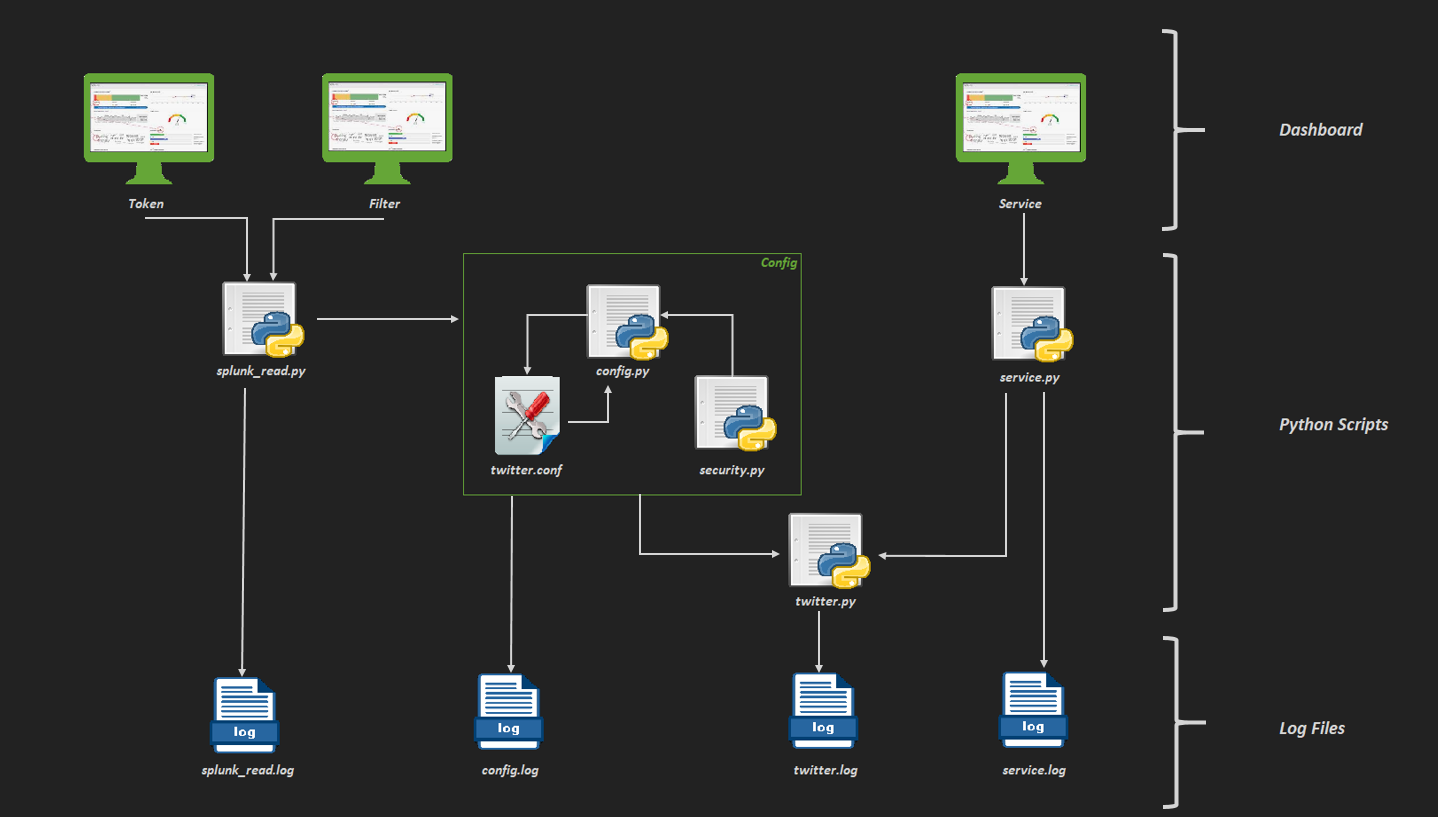
\includegraphics[scale=0.33]{img/arquitectura.PNG}
	\caption{\color{text}JPE\_Twitter General Diagram}
\end{figure}

\textit{\small \textbf{Importante:} Todas las librer\'ias necesarias para el correcto funcionamiento del aplicativo, se encuentran incluidas en el paquete de instalaci\'on}
\newpage
\subsection{Dashboards}

Para la administraci\'on del proceso de escucha de Twitter existen tres dashboard importantes, que permiten configurar los token de autentificaci\'on, configurar los filtros correspondientes e iniciar, detener, reiniciar o verificar el estado del servicio:
\newline
\begin{itemize}
\item Token and Security
\item Filter
\item Service
\newline
\end{itemize}

Además, cuenta con tres dashboard básicos que permiten visualizar información general de Twitter, en base a los filtros aplicados, tales como: usuario con más seguidores, hashtags más usados y usuarios mencionados: 
\newline
\begin{itemize}
\item Twitter Users
\item Twitter Hashtag
\item Twitter Comments
\newline
\end{itemize}

\subsubsection{Token and Security}

Este dashboard permite configurar los token de autenticaci\'on de la API de Twitter, los cuales son: \textit{consumer key, consumer secret, access token y access secret}. Estos token quedan almacenados en el archivo de configuraci\'on \textit{twitter.conf} y en lo que a seguridad respecta, los token de autenticaci\'on pueden ser encriptados para evitar que terceros accedan a ellos, solo es necesario escribir una clave de encriptaci\'on en el mismo panel, luego de indicar que deseas encriptar los token.
\newline
\begin{figure}[h!]
	\centering
	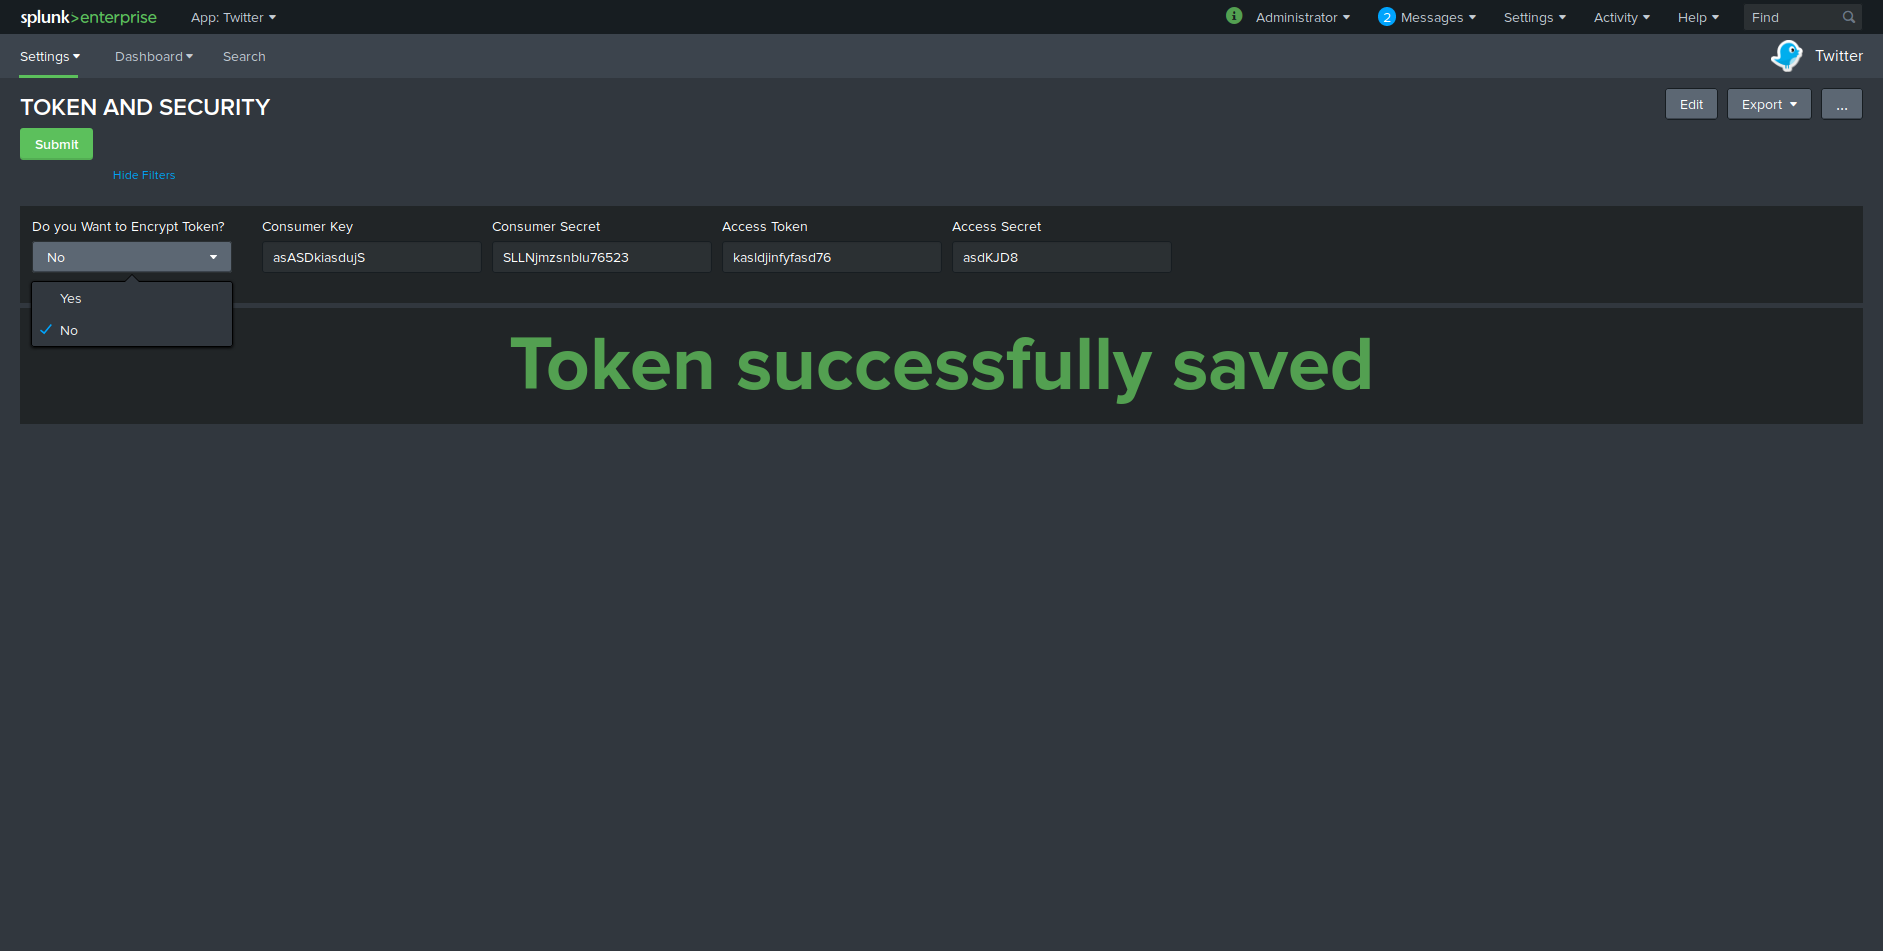
\includegraphics[scale=0.2]{img/token.png}
	\caption{\color{text}Setting: Token and Security Dashboard}
\end{figure}

Es importante considerar que: para obtener los token, se debe crear un cuenta de desarrollador en Twitter (\url{https://developer.twitter.com})
\newpage
\subsubsection{Filter}

Este dashboard permite configurar los filtros que se aplicar\'an en el proceso de escucha. Las opciones de configuraci\'n incluyen la acci\'on de agregar nuevo filtro al que se encuentra actualmente configurado o configurar nuevos filtros reemplazando a los anteriores, mediante la elecci\'on de \textit{add o new} respectivamente.\\ Los filtros ingresados pueden ser palabras, frases, hashtag, entre otros y deben ser separados por una coma.
\newline
\begin{figure}[h!]
	\centering
	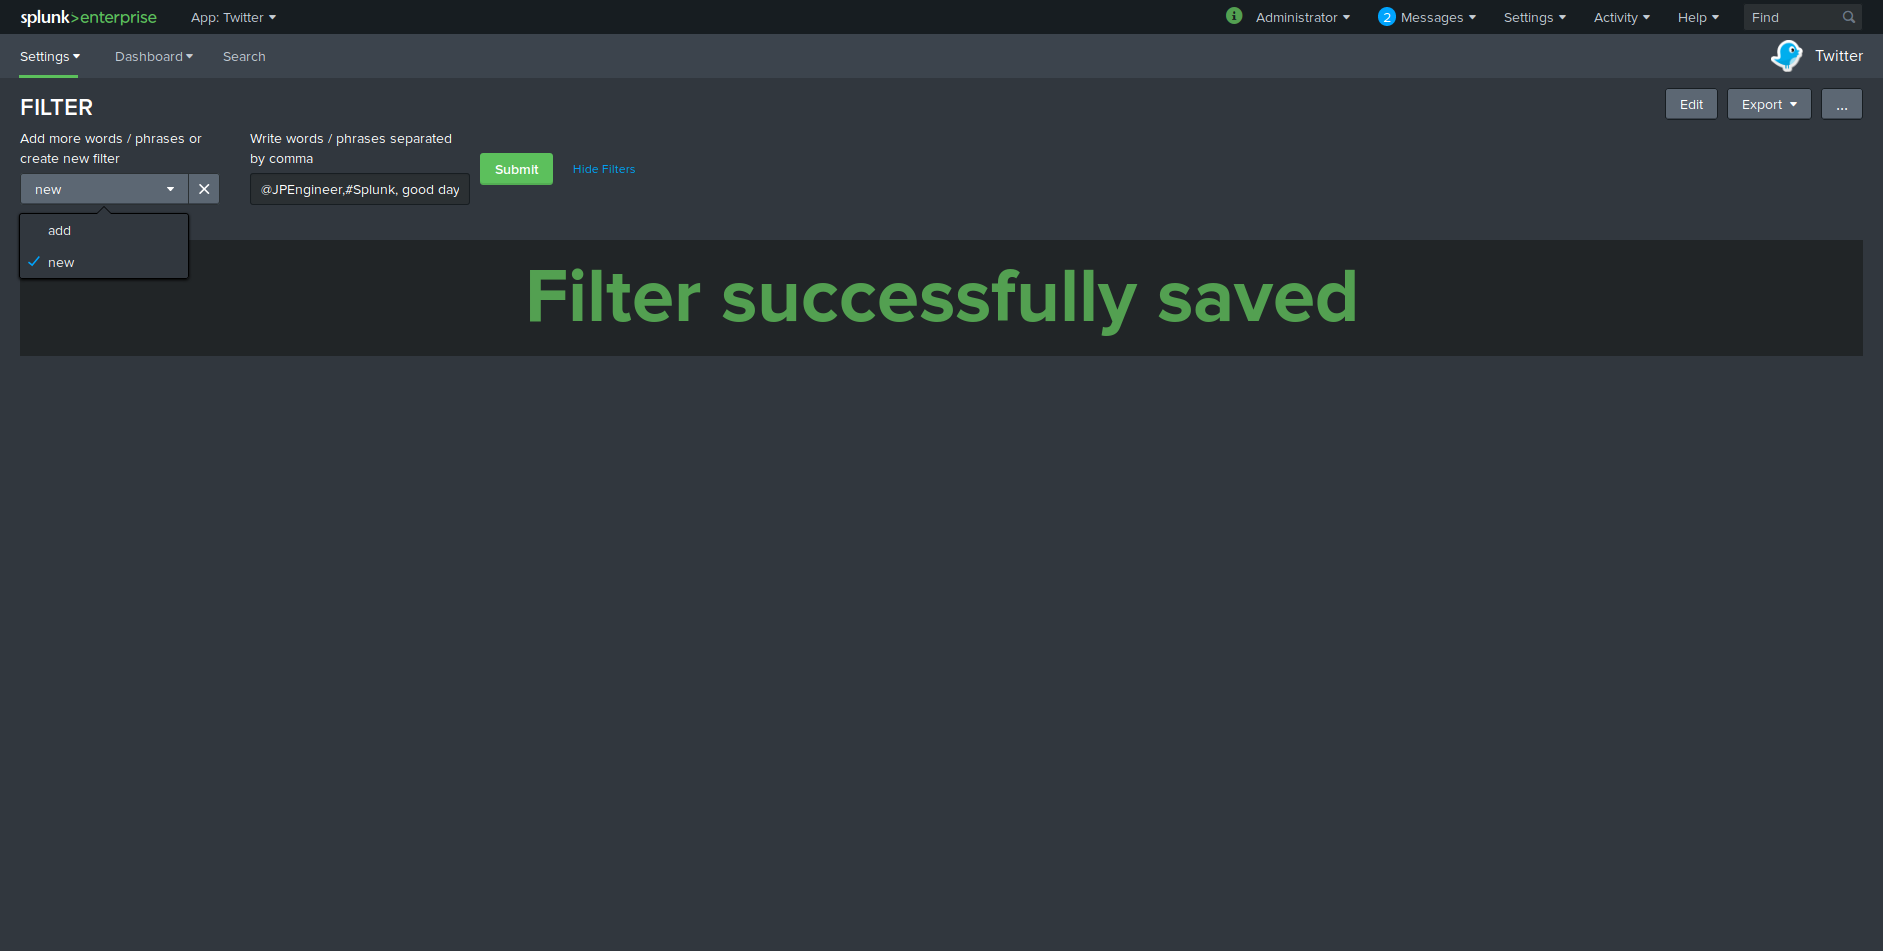
\includegraphics[scale=0.2]{img/filter.png}
	\caption{\color{text}Setting: filter Dashboard}
\end{figure}

\subsubsection{Service}

Este dashboard permite ejecutar acciones sobre el servicio de Twitter. La opción Start permite iniciar el servicio y comenzar a indexar data obtenida desde Twitter y como requisito previo, se requiere tener configurado los Token de autenticación y los filtros. La opción Stop es la encargada de detener el servicio. La opción Restart permite reiniciar el servicio si es requerido por desarrollos propios u otras razones. La opcion Status indica si el servicio se encuentra activo o detenido.
\newline
\begin{figure}[h!]
	\centering
	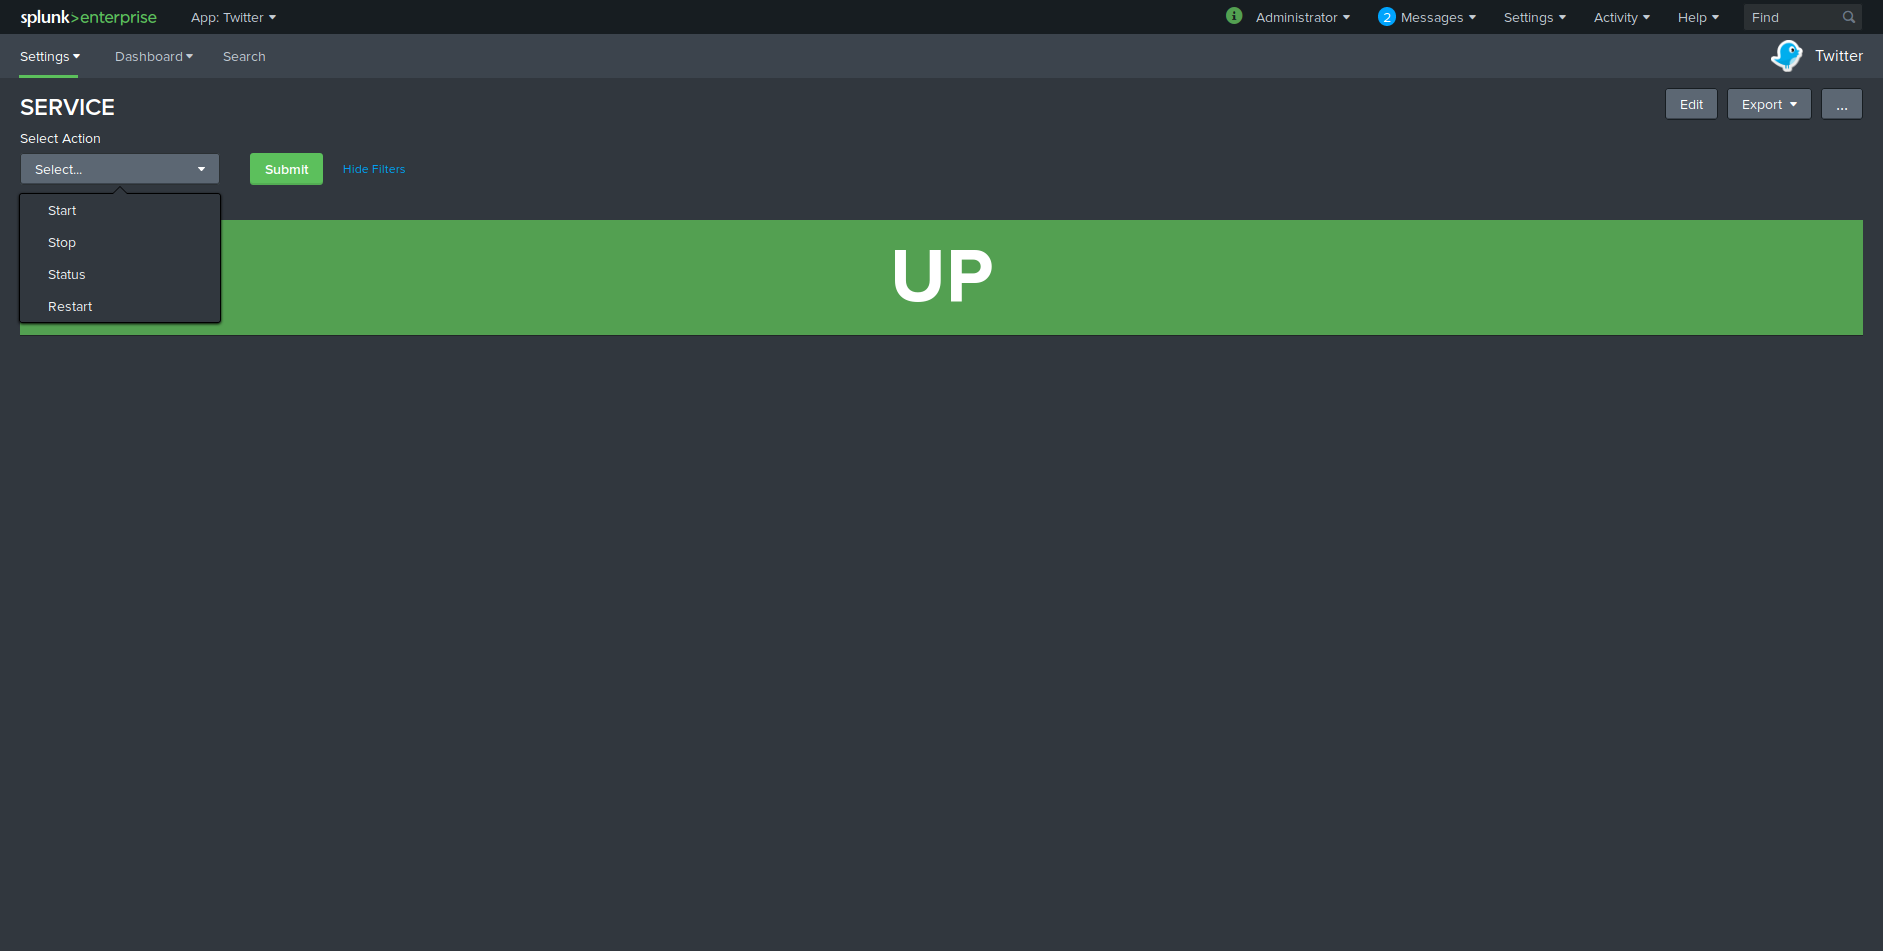
\includegraphics[scale=0.2]{img/service.png}
	\caption{\color{text}Setting: Service Dashboard}
\end{figure}


\subsubsection{Twitter Users}

Este dashboard presenta información relacionada a usuarios de la red social, tales como: cantidad de seguidores, nombre, alias y ubicación. Sobre el mismo dashboard se pueden aplicar desarrollos para obtener informaci\'on adicional.
\newline
\begin{figure}[h!]
	\centering
	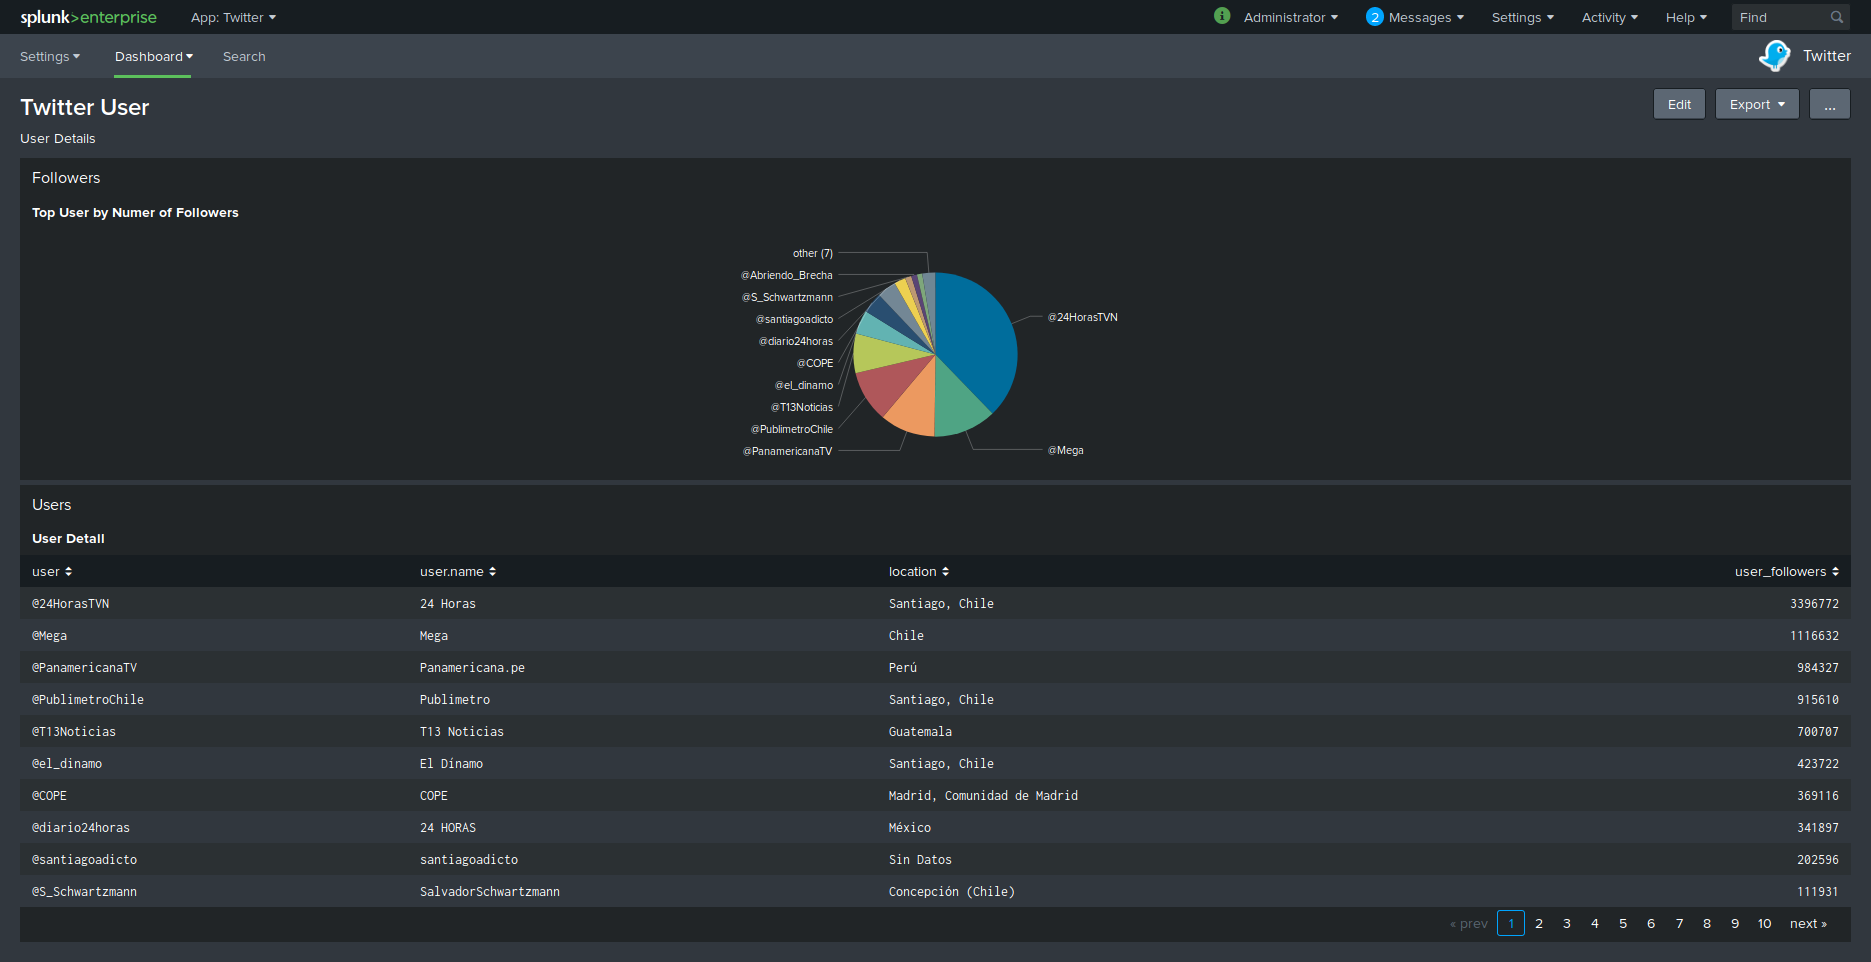
\includegraphics[scale=0.2]{img/user.png}
	\caption{\color{text}Twitter User Dashboard}
\end{figure}

\subsubsection{Twitter Hashtag}

Este dashboard presenta informaci\'on relacionada a los hashtag m\'as usados durante el d\'ia. Sobre el mismo dashboard se pueden aplicar desarrollos para obtener informaci\'on adicional.
\newline
\begin{figure}[h!]
	\centering
	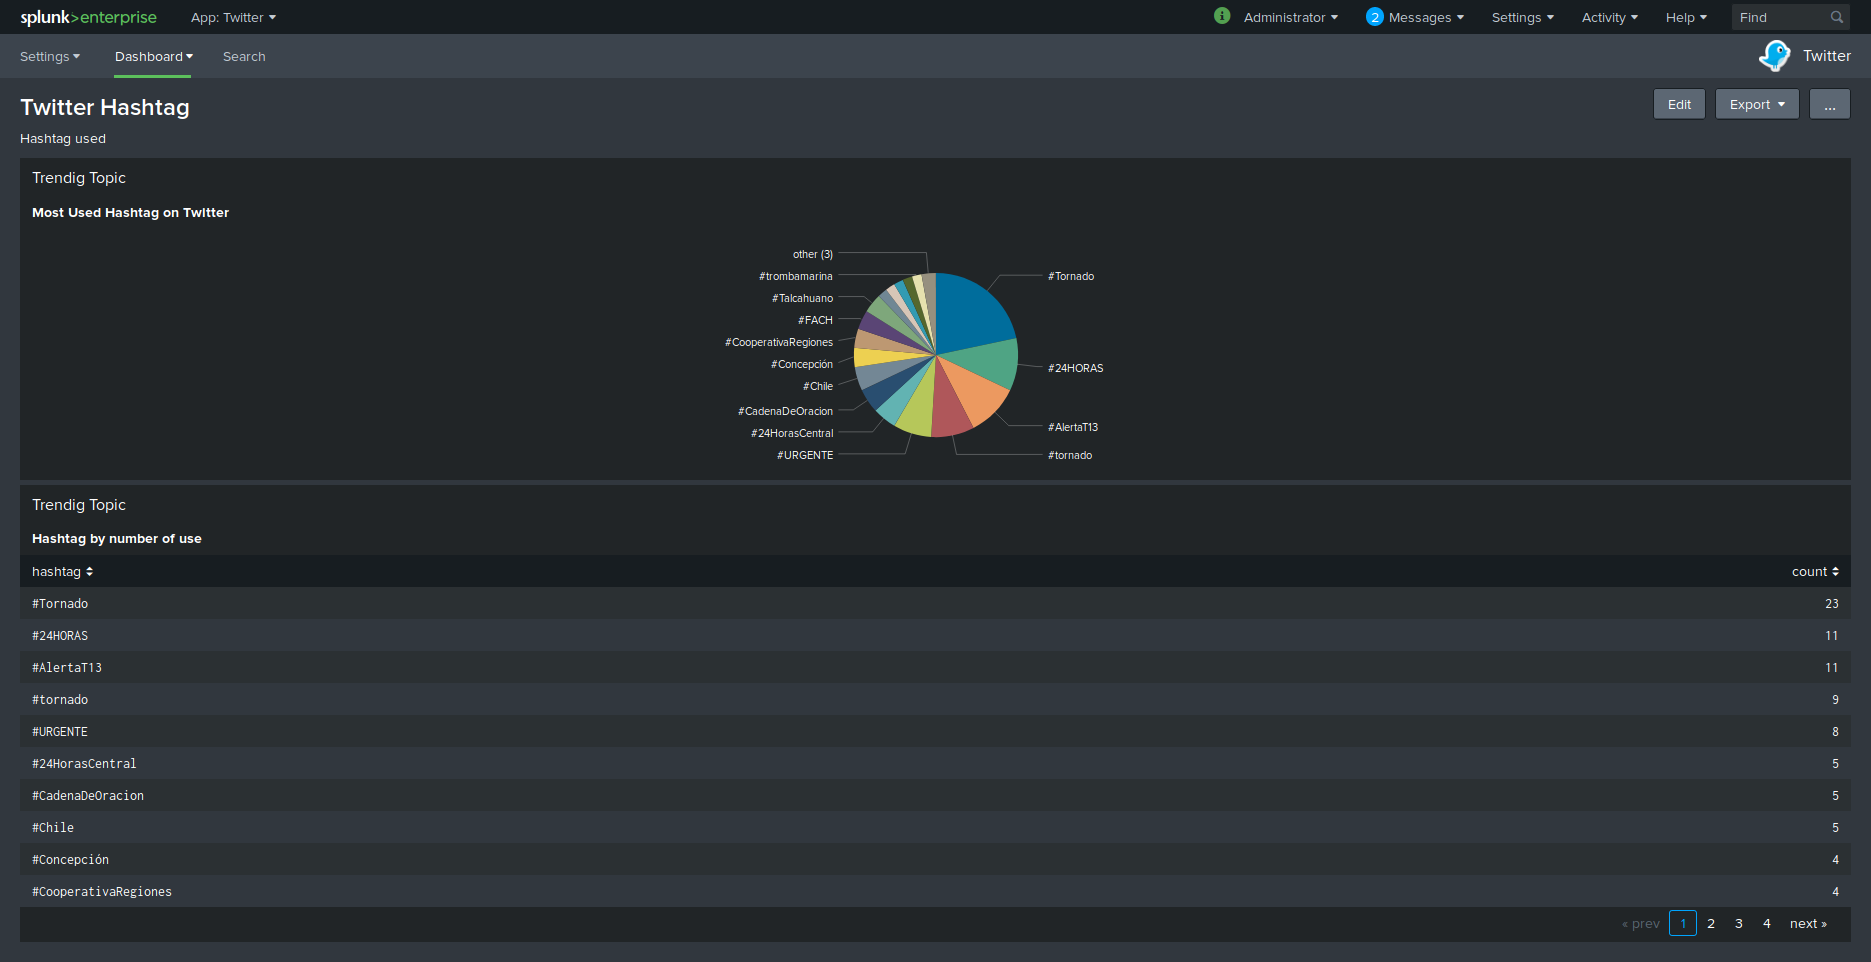
\includegraphics[scale=0.2]{img/hashtag.png}
	\caption{\color{text}Twitter Hashtag Dashboard}
\end{figure}

\newpage

\subsubsection{Twitter Comments}

Esta dashboard presenta el detalle de los usuarios m\'as comentados del d\'ia, comentarios realizados e informaci\'on del usuario. Sobre el mismo dashboard se pueden aplicar desarrollos para obtener informaci\'on adicional.
\newline
\begin{figure}[h!]
	\centering
	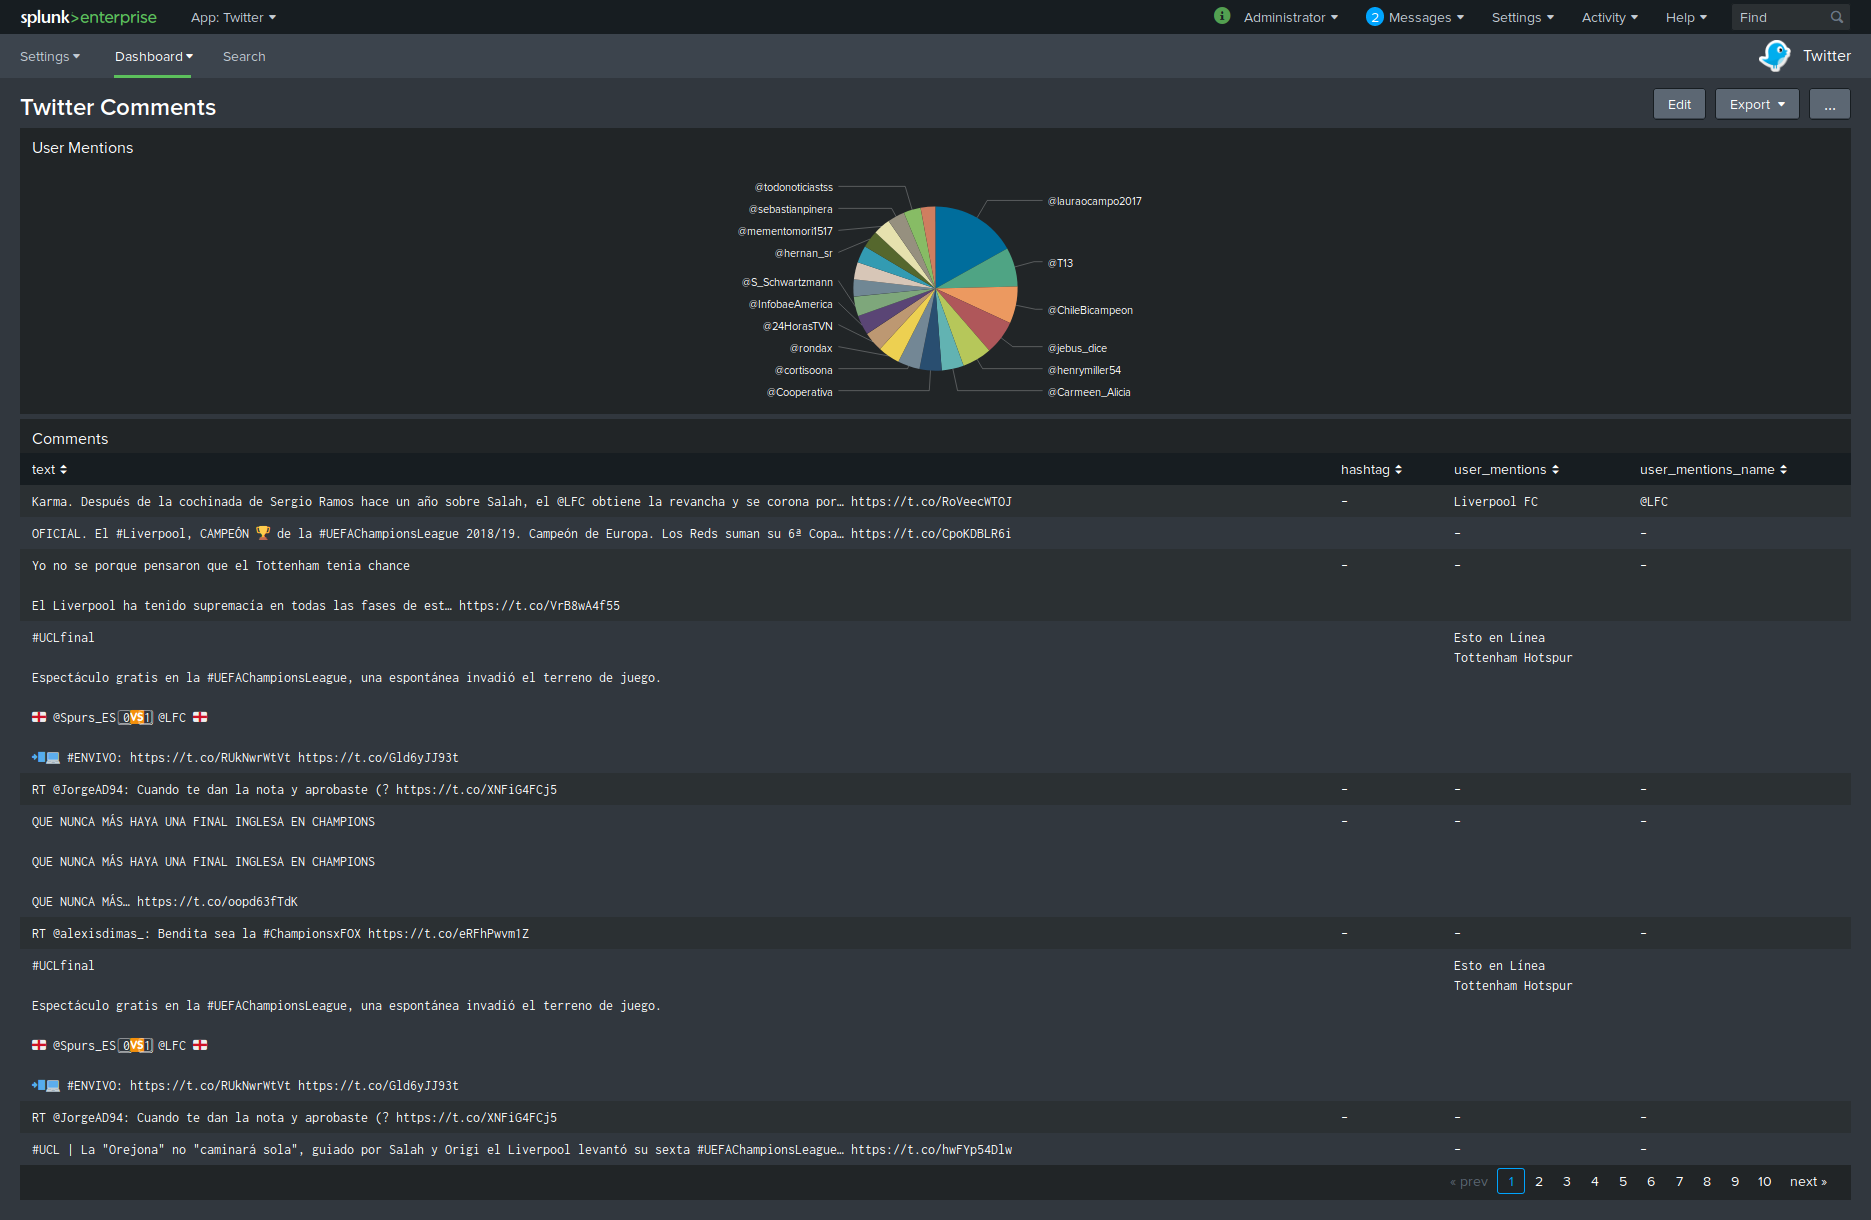
\includegraphics[scale=0.2]{img/comments.png}
	\caption{\color{text}Twitter Comments Dashboard}
\end{figure}

\newpage

\section{Instalaci\'on}

JPE\_Twitter esta probado en versiones 6.x de Splunk o superior y fue desarrollado en Splunk 7, el cual ser\'a usado en la gu\'ia de instalaci\'on.\\
\\
Considerando que la aplicaci\'on ya se encuentra descargada, debes seguir los siguuentes pasos:
\newline
\begin{enumerate}[label=(\alph*)]
\item Hacer click en el apartado superi\'or izquierdo de la plataforma Splunk, que dice \textbf{App: Search \& Reporting} > \textbf{Manage Apps}
\item Hacer click en el extremo superior derecho de la plataforma, en el bot\'on \textbf{Install Apps from File}
\item Hacer click en \textbf{Examine} y seleccionar JPE\_Twitter.zip, luego hacer click en \textbf{Upload}
\newline
\end{enumerate}

\begin{figure}[h!]
  \centering
  \begin{subfigure}[b]{0.49\linewidth}
    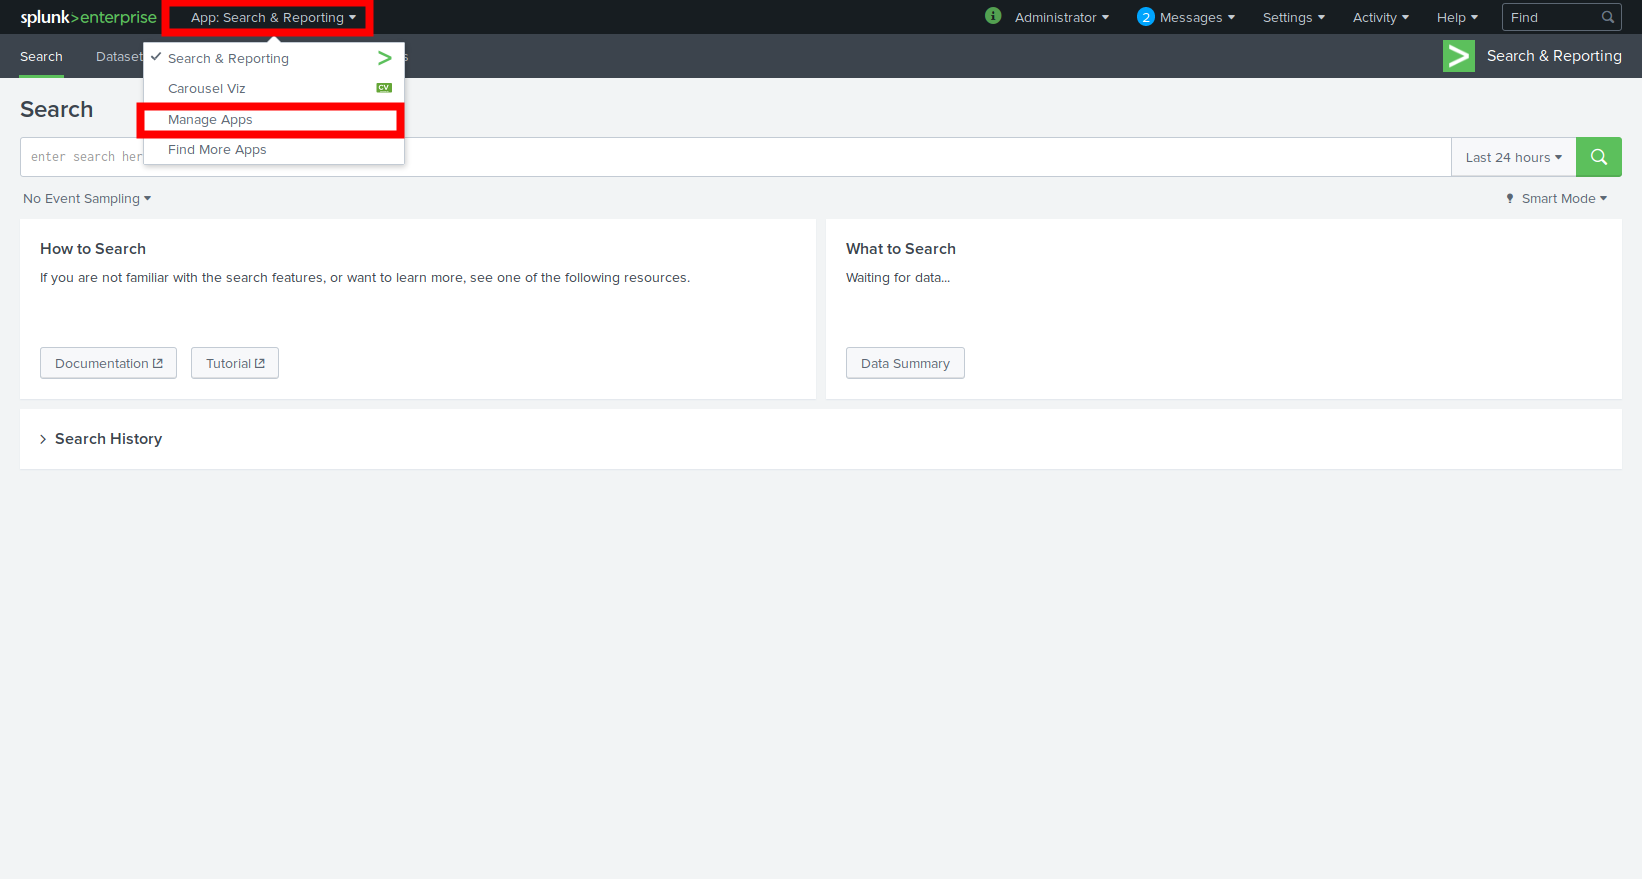
\includegraphics[width=\linewidth]{img/a.png}
     \caption{\color{text} Manage Apps}
  \end{subfigure}
  \begin{subfigure}[b]{0.49\linewidth}
    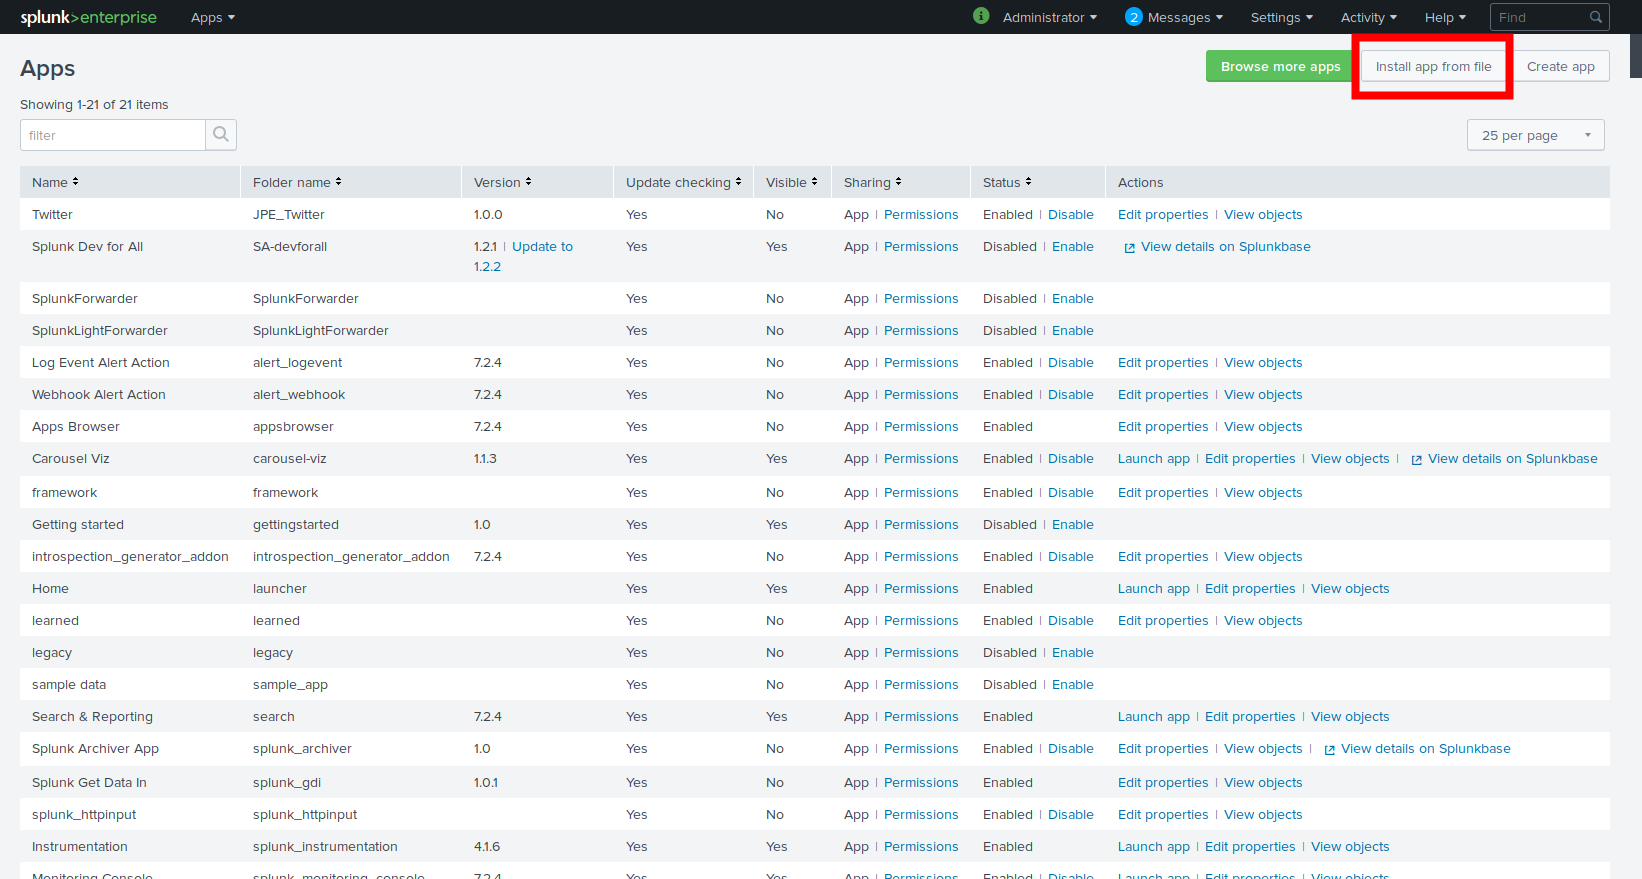
\includegraphics[width=\linewidth]{img/b.png}
    \caption{\color{text} Install Apps from File}
  \end{subfigure}
  \begin{subfigure}[b]{0.49\linewidth}
    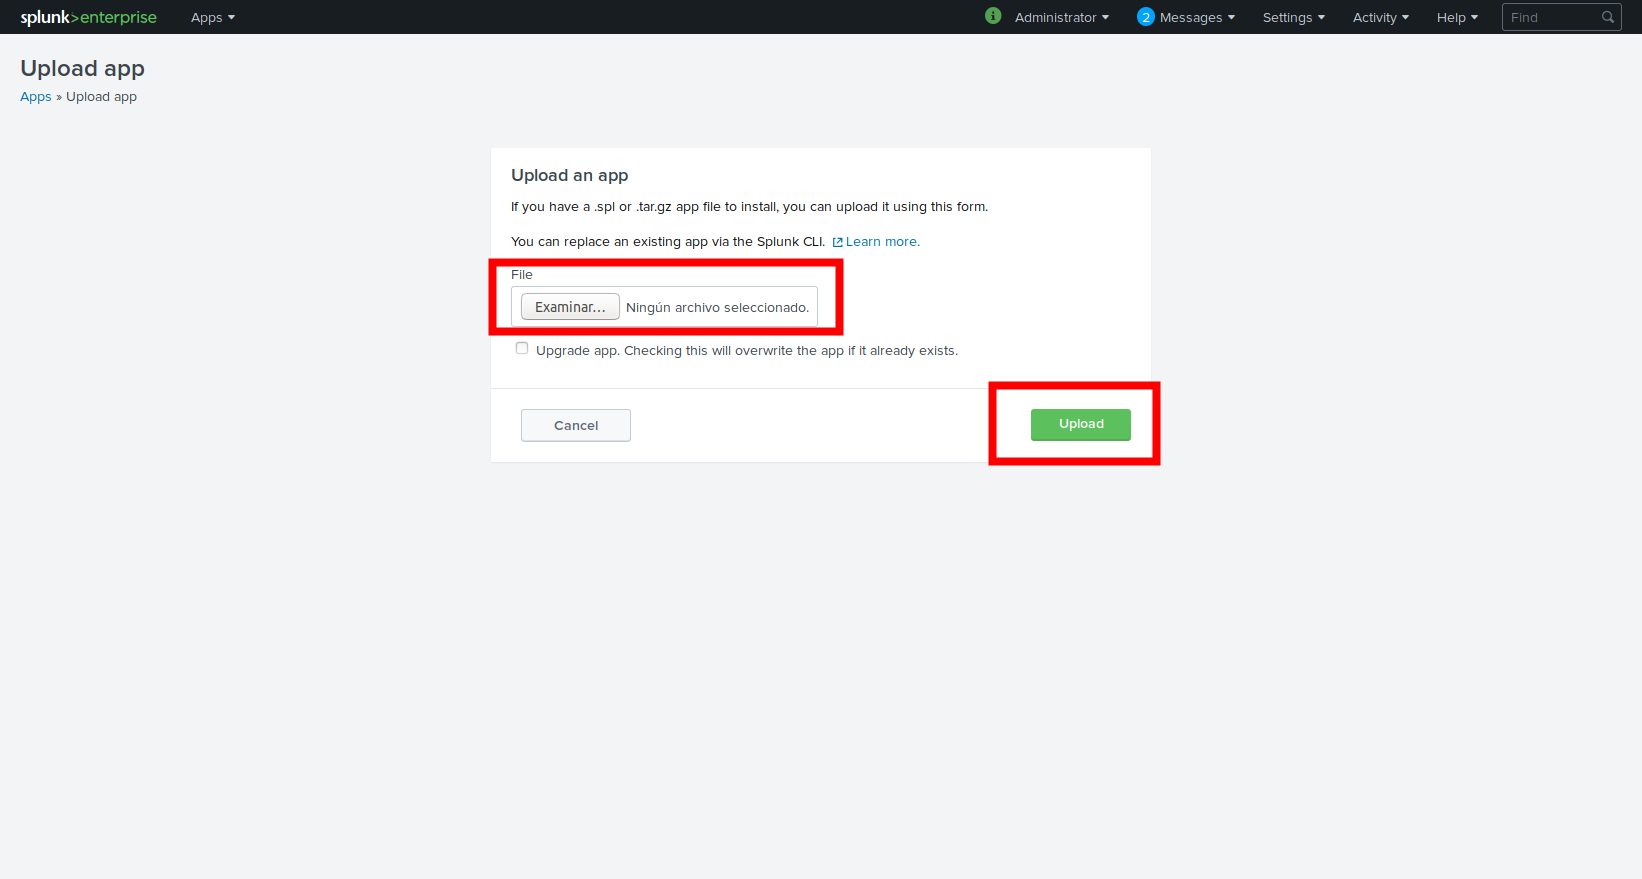
\includegraphics[width=\linewidth]{img/c.png}
    \caption{\color{text} Upload}
  \end{subfigure}
  \caption{\color{text} Instalaci\'on de la aplicaci\'on JPE\_Twitter}
  \label{fig:instalacion}
\end{figure}

Con estos simples pasos, JPE\_Twitter se encontrar\'a instalado. La recomendaci\'on pos-instalaci\'on es reiniciar Splunk.
\newpage
\section{Validaciones}

Para la validaci\'on de la instalaci\'on se deben seguir los siguientes pasos:
\newline

\begin{enumerate}[label=(\alph*)]
\item Hacer click en el apartado superior derecho de la plataforma, en la secci\'on \textbf{Setting > Indexes}
\item Validar que exista el index \textbf{twitter}
\item Hacer click en \textbf{Setting > Source Types} y validar que existan los source types \textbf{twitter, setting} y \textbf{service}
\newline
\end{enumerate}

\begin{figure}[h!]
  \centering
  \begin{subfigure}[b]{0.49\linewidth}
    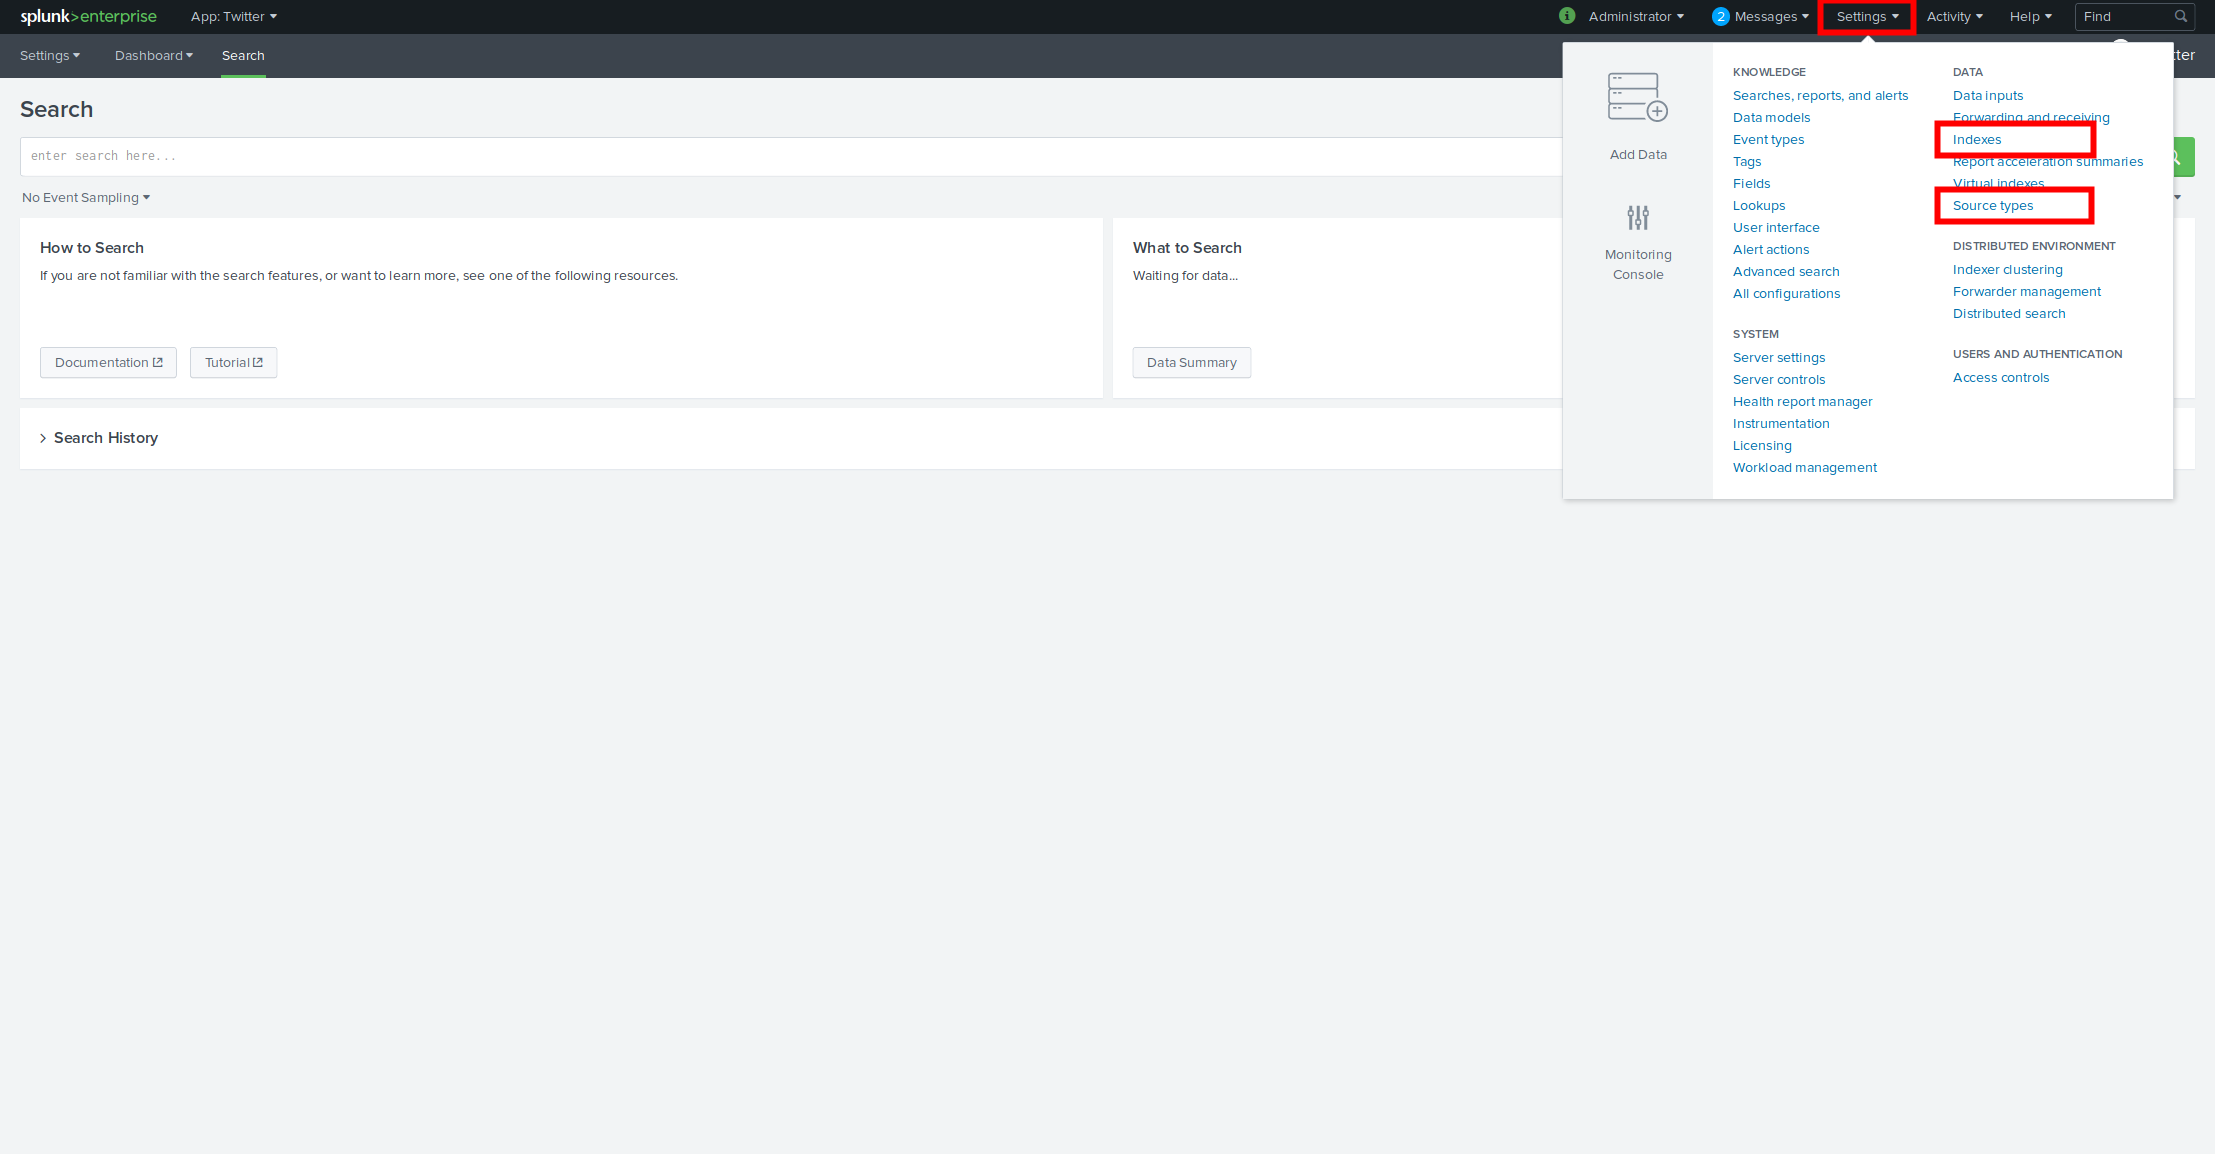
\includegraphics[width=\linewidth]{img/f.png}
     \caption{\color{text} Setting: Index - Sourcetype}
  \end{subfigure}
  \begin{subfigure}[b]{0.49\linewidth}
    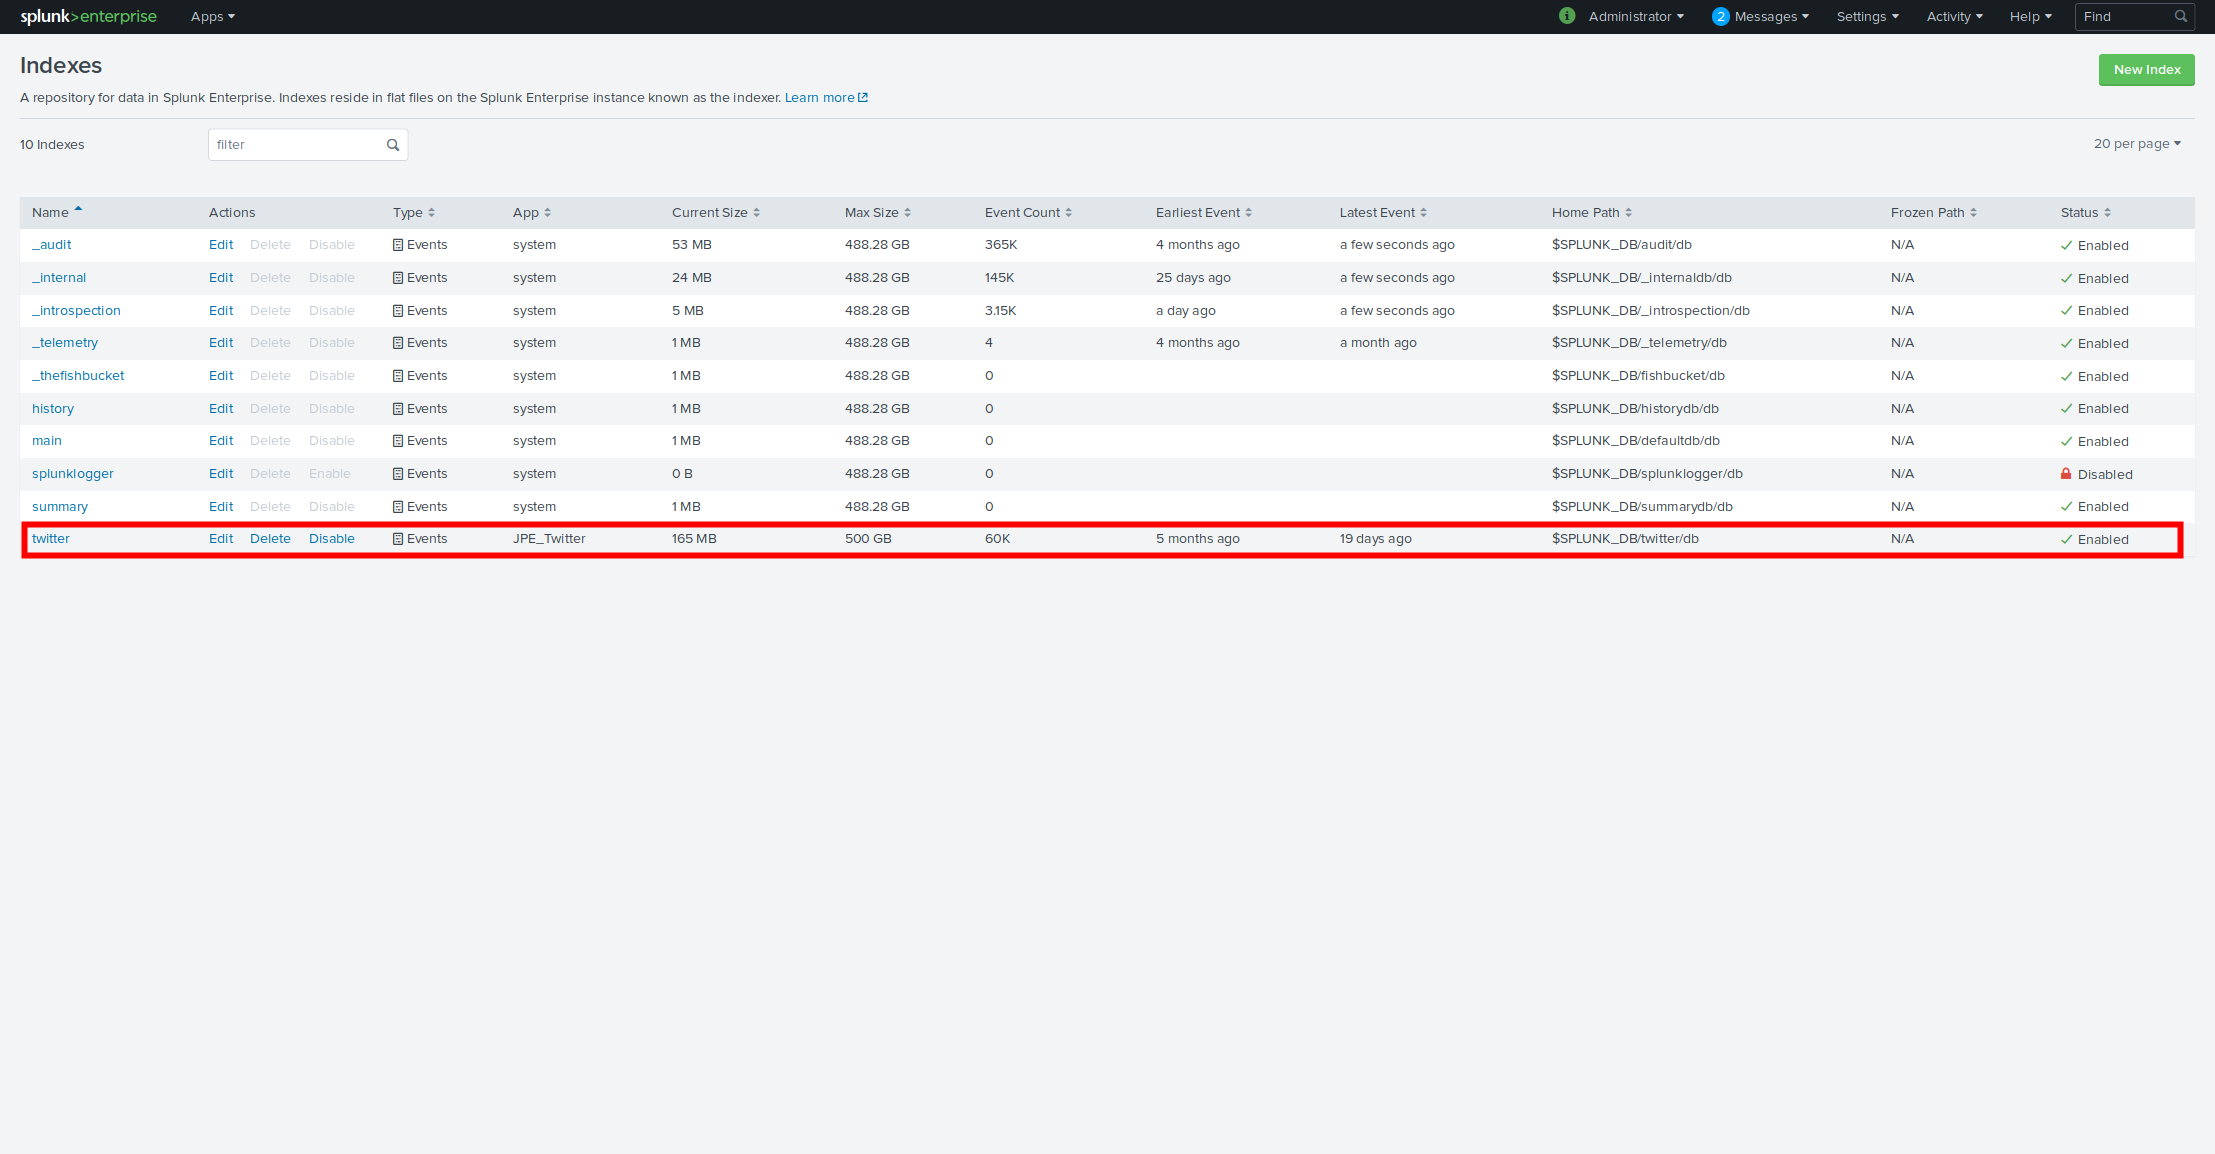
\includegraphics[width=\linewidth]{img/d.png}
    \caption{\color{text} Index}
  \end{subfigure}
  \begin{subfigure}[b]{0.49\linewidth}
    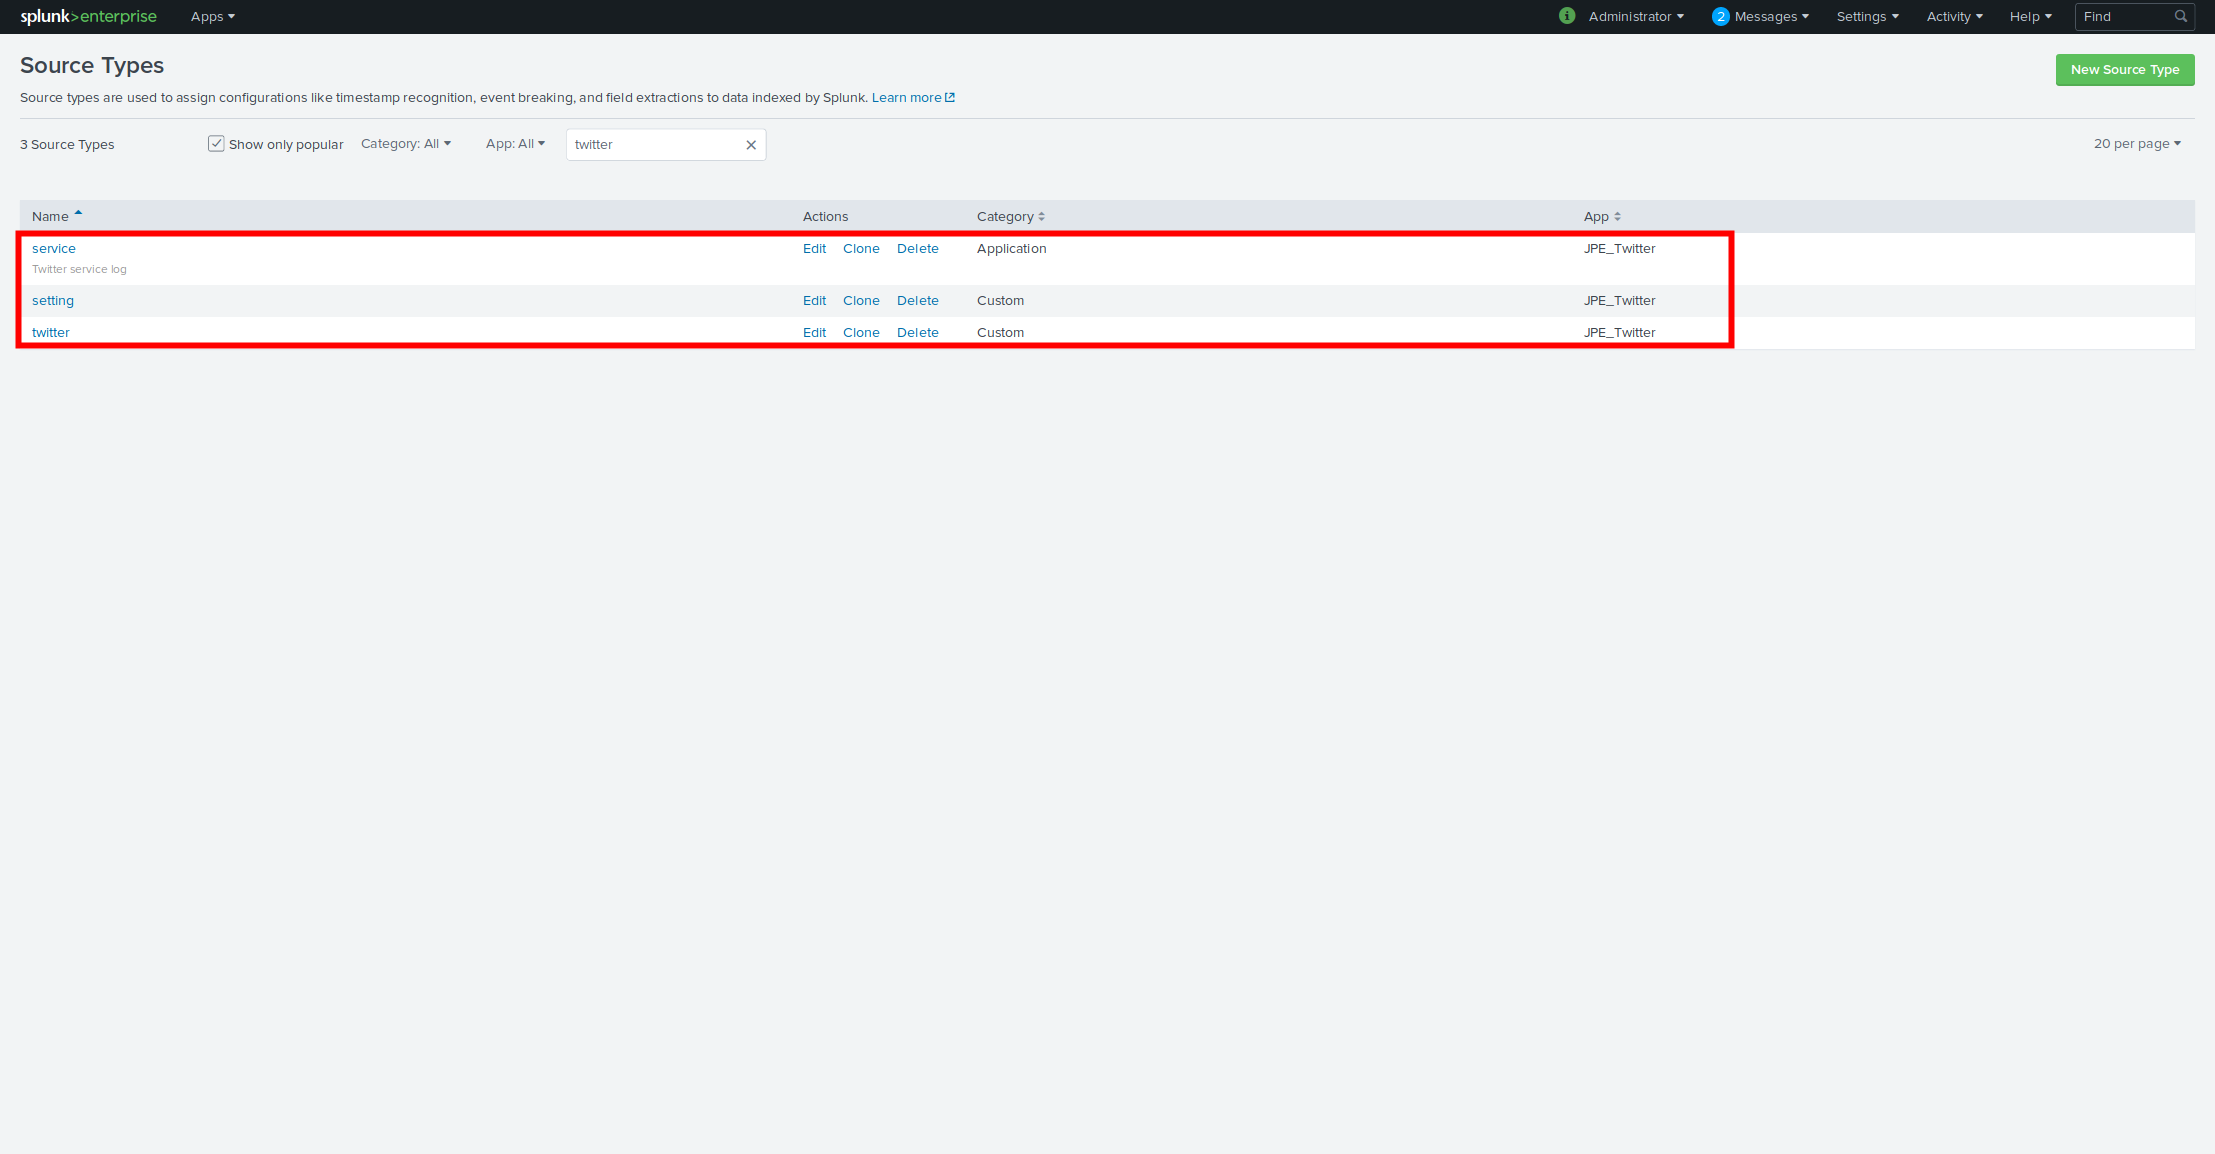
\includegraphics[width=\linewidth]{img/e.png}
    \caption{\color{text} Sourcetype}
  \end{subfigure}
  \caption{\color{text} Validaciones}
  \label{fig:validacion}
\end{figure}

\textbf{Index twitter: }Es el repositorio de datos del aplicativo instalado.\\
\textbf{Source Type twitter: }Identifica la estructura de los datos filtrados de Twitter.\\
\textbf{Source Type service: }Identifica la estructura de los datos generador por el m\'odulo \textit{service.py}\\
\textbf{Source Type setting: }Identifica la estructura de los datos generador por los m\'odulos \textit{twitter.py} y \textit{security.py}
\newline
\section{Soporte, consultas o comentarios}

\textbf{Nombre: }Juan Alejandro P\'erez Chand\'ia\\
\textbf{E-Mail: }jalejandro.ingeniero@gmail.com\\
\textbf{Idioma: }Espa\~nol - Ingl\'es
% \end{large}
\end{document}
